\chapter{Future Work: Large Scale Analysis of Multi-Site Preclinical Alzheimer's Disease} \label{chap:pac} 

With the above tools in hand, we aim to move towards applying and deploying both conditional independence schemes and efficient EMD-fairness methods to 
the analysis of a new preclinical cohort of individuals at risk for developing Alzheimer's disease.

\textbf{Data.} Here our data consists of patient information pooled across multiple sites. Demographic measures, neuropsychological test results, genetic indicators, and cerebrospinal fluid (CSF) biomarkers were all collected on individuals from three studies: the Adult Children Study (ACS), the Wisconsin Registry for Alzheimer's Prevention (WRAP), and the Biomarkers of Cognitive Decline Among Normal Individuals (BIOCARD). Data was preprocessed using standard pipelines, collated, and harmonized across sites. Table~\ref{tab:pacfeats} details the full list of measures.

\begin{table}
    \centering
    \begin{tabular}{l|l}
        \hline\hline
         A$\beta$42 & A$\beta$40 \\
         T-Tau & P-Tau \\
         A$\beta$42/A$\beta$40 & PTAU-A$\beta$42 \\
         Age & Gender \\
         Executive Function & General Cognitive Performance \\
         Episodic Memory & Time \\
         Education & APOE \\
         \hline\hline
    \end{tabular}
    \caption{Preclinical AD Measures used in conditional independence analysis.}
    \label{tab:pacfeats}
\end{table}

Imaging data is also available for a subset of the individuals included in the above set, and future work includes incorporation of these imaging modalities (MRI, DTI, and PET region of interest measures).

\textbf{Methods.} The results shown here demonstrate the potential value of applying conditional independence methods over standard correlation methods. 

\begin{figure}
    \centering
    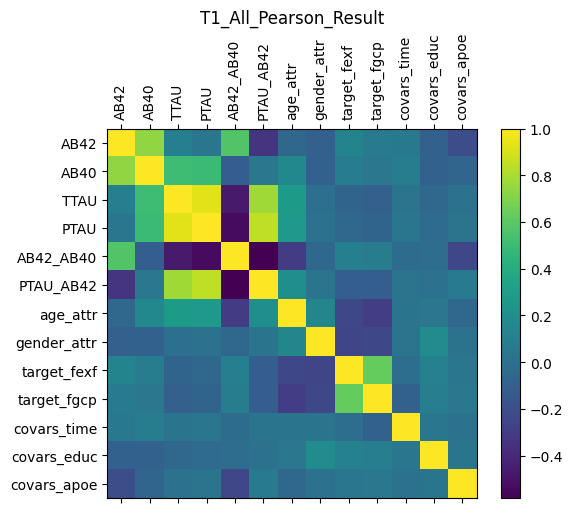
\includegraphics[width=0.24\textwidth]{chap6/figs/T1_All_Pearson_Result.png}
    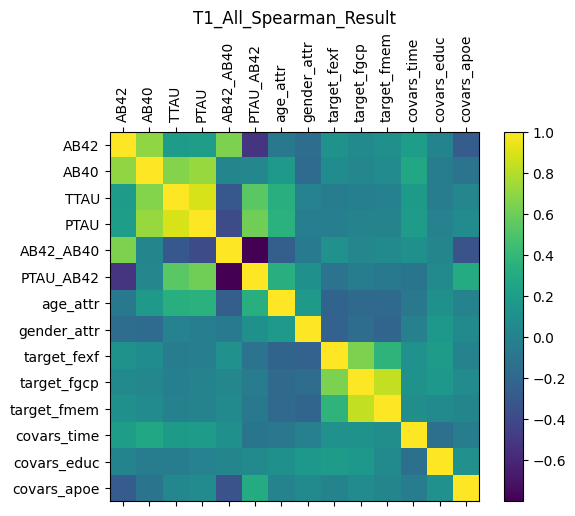
\includegraphics[width=0.24\textwidth]{chap6/figs/T1_All_Spearman_Result.png}
    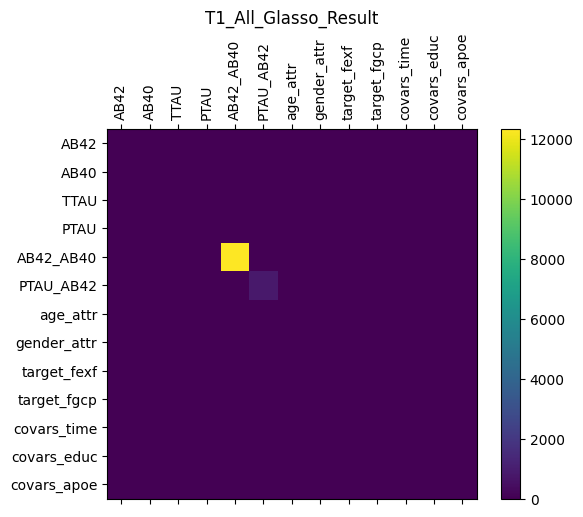
\includegraphics[width=0.24\textwidth]{chap6/figs/T1_All_Glasso_Result.png}
    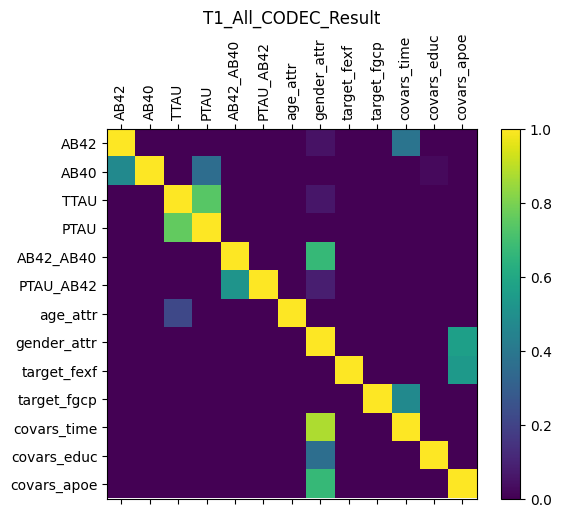
\includegraphics[width=0.24\textwidth]{chap6/figs/T1_All_CODEC_Result.png}
    
    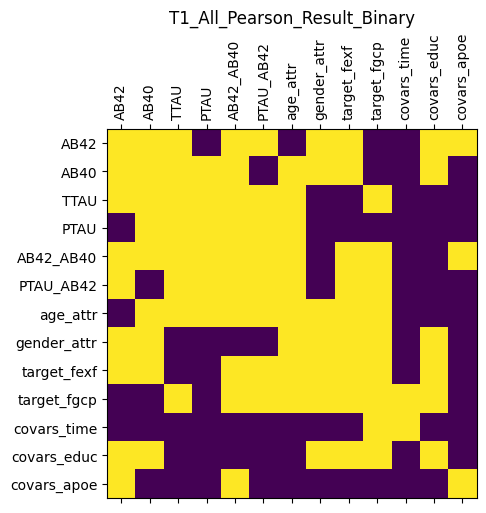
\includegraphics[width=0.24\textwidth]{chap6/figs/T1_All_Pearson_Result_Binary.png}
    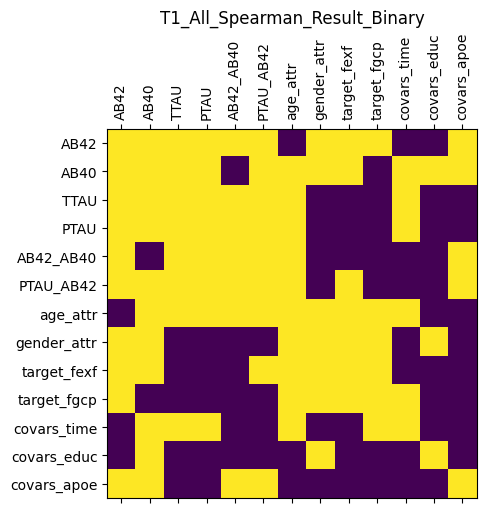
\includegraphics[width=0.24\textwidth]{chap6/figs/T1_All_Spearman_Result_Binary.png}
    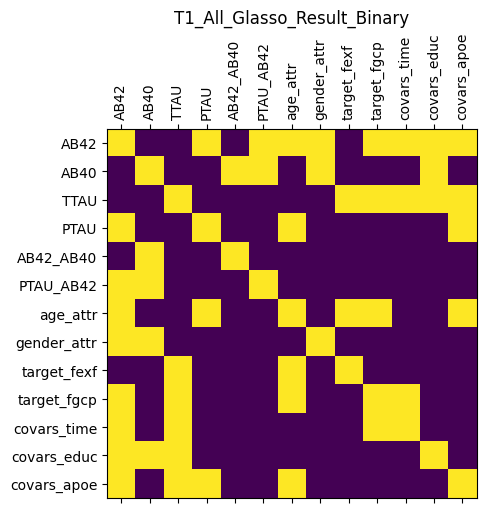
\includegraphics[width=0.24\textwidth]{chap6/figs/T1_All_Glasso_Result_Binary.png}
    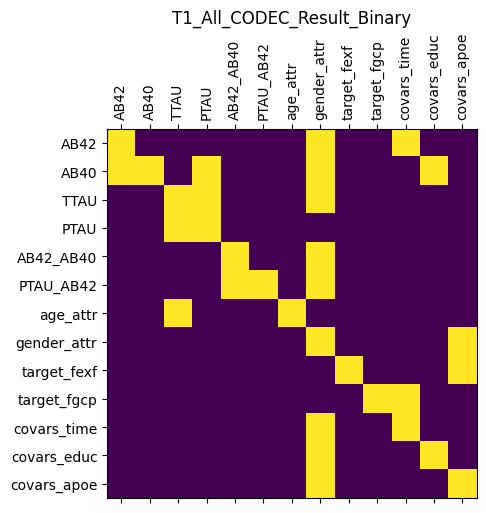
\includegraphics[width=0.24\textwidth]{chap6/figs/T1_All_CODEC_Result_Binary.png}
    \caption{All Sites.}
    \label{fig:all}
\end{figure}

\begin{figure}
    \centering
    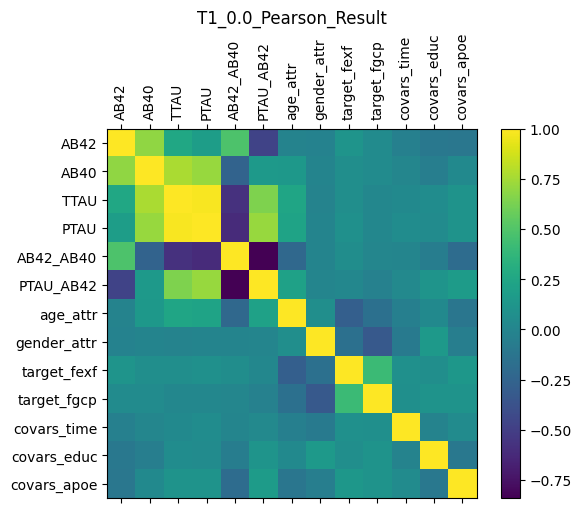
\includegraphics[width=0.24\textwidth]{chap6/figs/T1_0.0_Pearson_Result.png}
    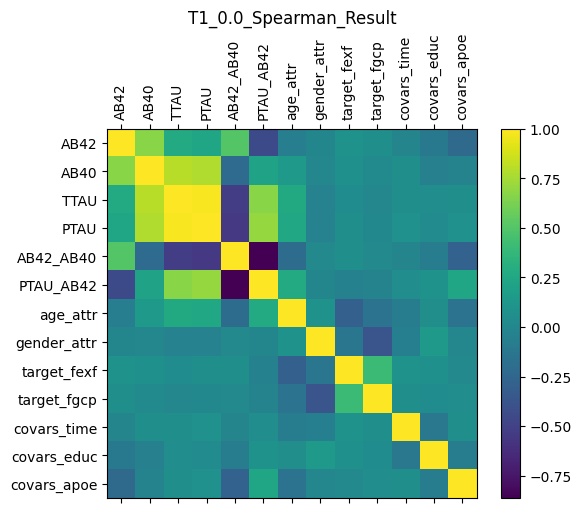
\includegraphics[width=0.24\textwidth]{chap6/figs/T1_0.0_Spearman_Result.png}
    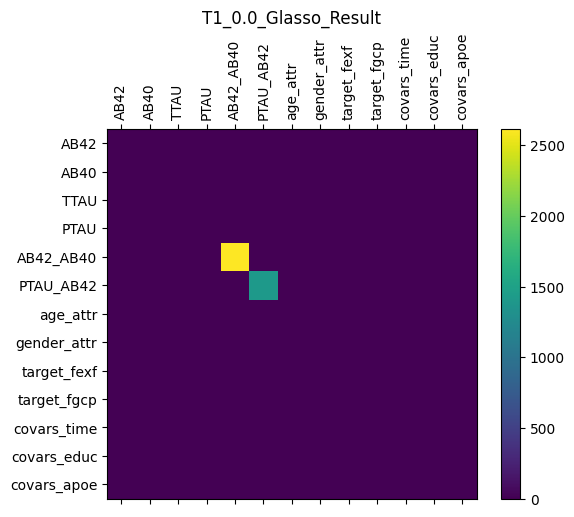
\includegraphics[width=0.24\textwidth]{chap6/figs/T1_0.0_Glasso_Result.png}
    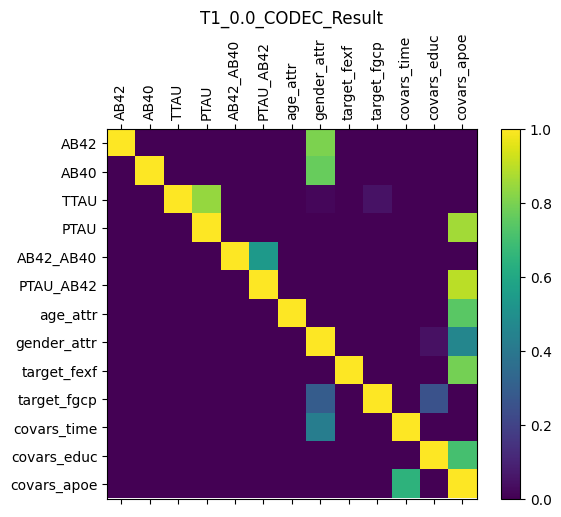
\includegraphics[width=0.24\textwidth]{chap6/figs/T1_0.0_CODEC_Result.png}
    
    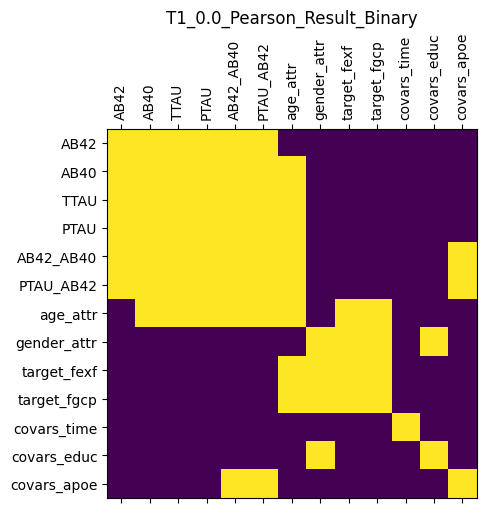
\includegraphics[width=0.24\textwidth]{chap6/figs/T1_0.0_Pearson_Result_Binary.png}
    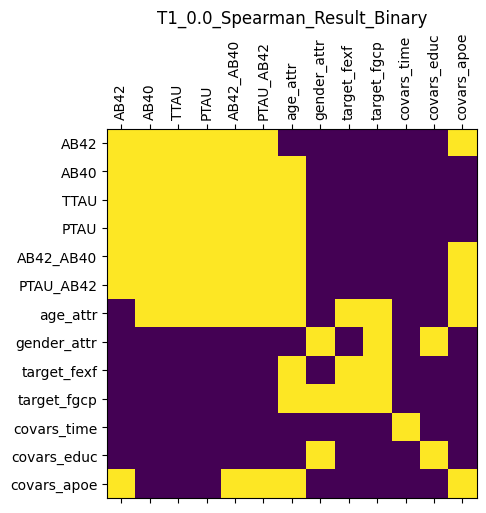
\includegraphics[width=0.24\textwidth]{chap6/figs/T1_0.0_Spearman_Result_Binary.png}
    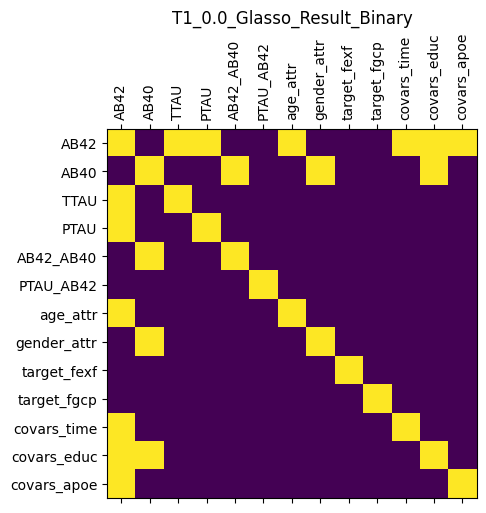
\includegraphics[width=0.24\textwidth]{chap6/figs/T1_0.0_Glasso_Result_Binary.png}
    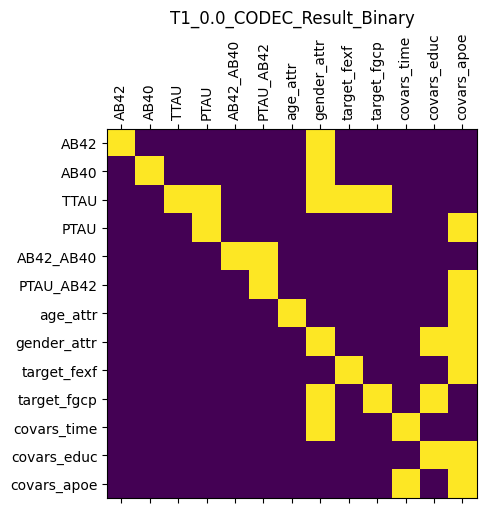
\includegraphics[width=0.24\textwidth]{chap6/figs/T1_0.0_CODEC_Result_Binary.png}
    \caption{Site 0: WRAP.}
    \label{fig:site0}
\end{figure}

\begin{figure}
    \centering
    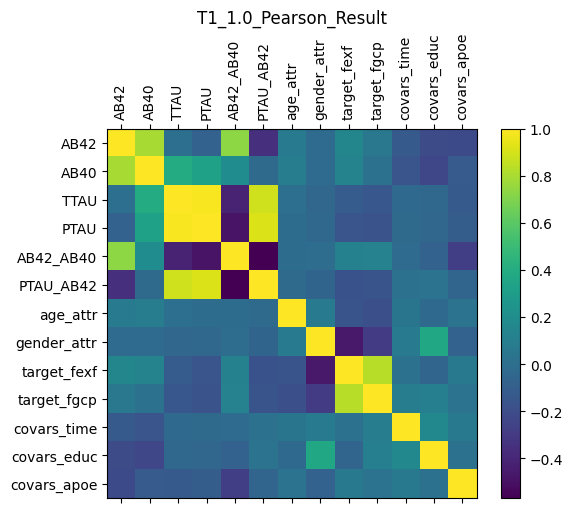
\includegraphics[width=0.24\textwidth]{chap6/figs/T1_1.0_Pearson_Result.png}
    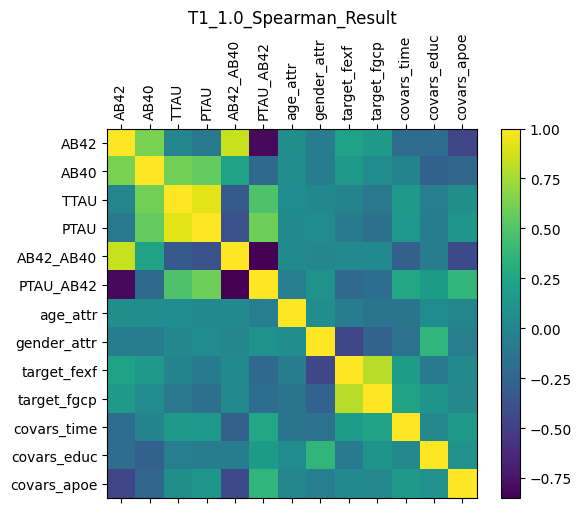
\includegraphics[width=0.24\textwidth]{chap6/figs/T1_1.0_Spearman_Result.png}
    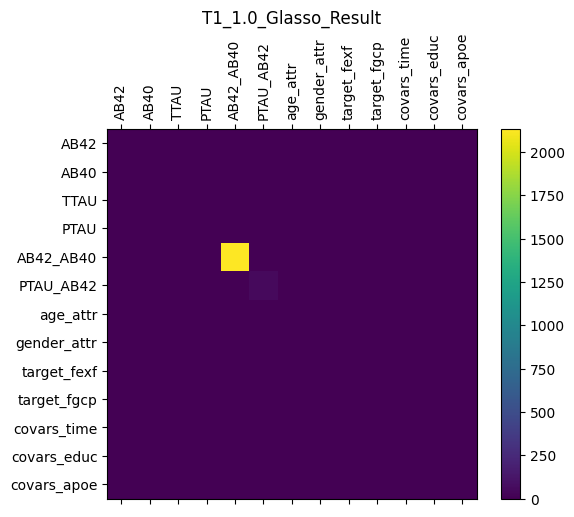
\includegraphics[width=0.24\textwidth]{chap6/figs/T1_1.0_Glasso_Result.png}
    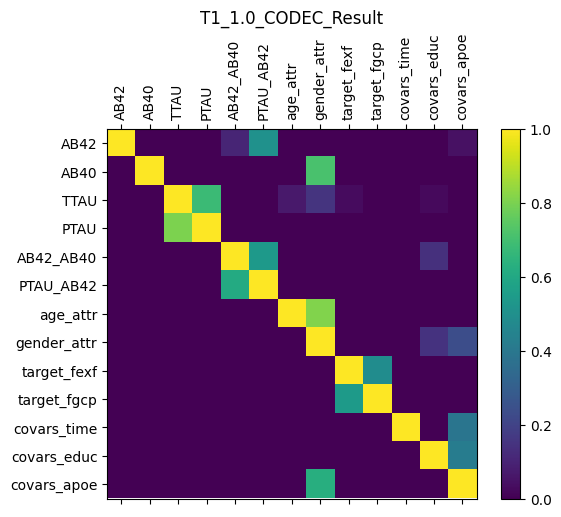
\includegraphics[width=0.24\textwidth]{chap6/figs/T1_1.0_CODEC_Result.png}
    
    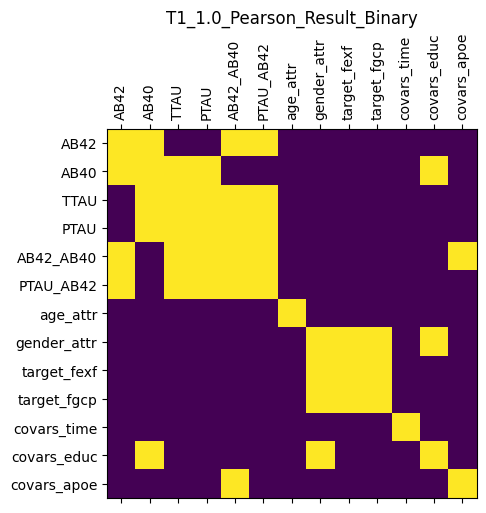
\includegraphics[width=0.24\textwidth]{chap6/figs/T1_1.0_Pearson_Result_Binary.png}
    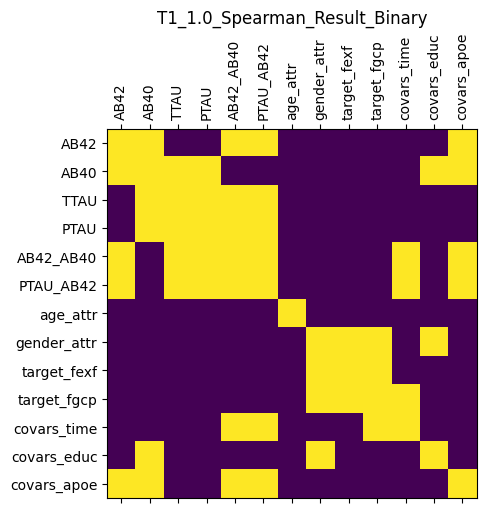
\includegraphics[width=0.24\textwidth]{chap6/figs/T1_1.0_Spearman_Result_Binary.png}
    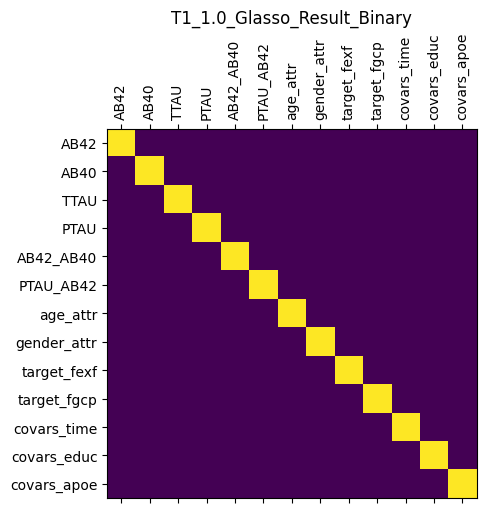
\includegraphics[width=0.24\textwidth]{chap6/figs/T1_1.0_Glasso_Result_Binary.png}
    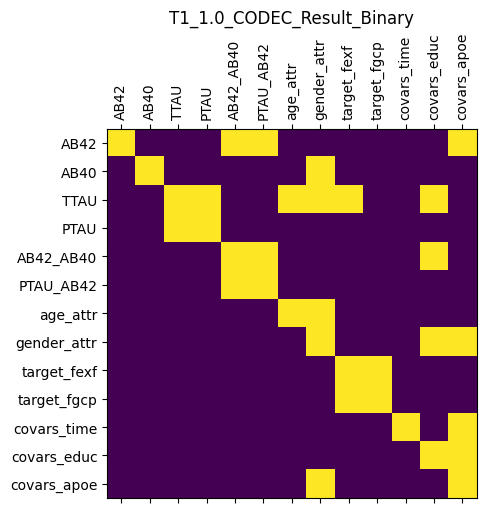
\includegraphics[width=0.24\textwidth]{chap6/figs/T1_1.0_CODEC_Result_Binary.png}
    \caption{Site 1: ACS.}
    \label{fig:site1}
\end{figure}

\begin{figure}
    \centering
    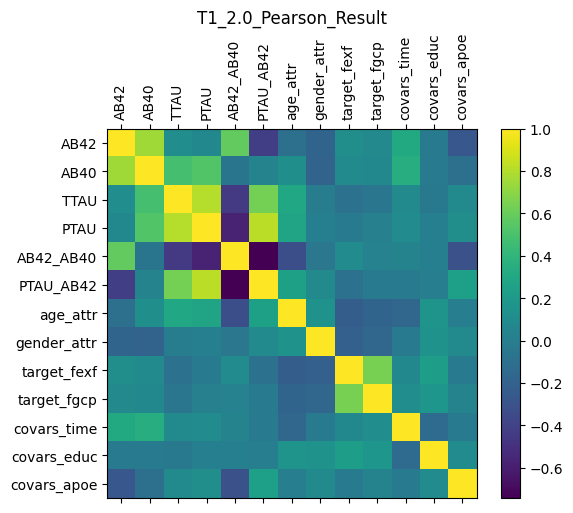
\includegraphics[width=0.24\textwidth]{chap6/figs/T1_2.0_Pearson_Result.png}
    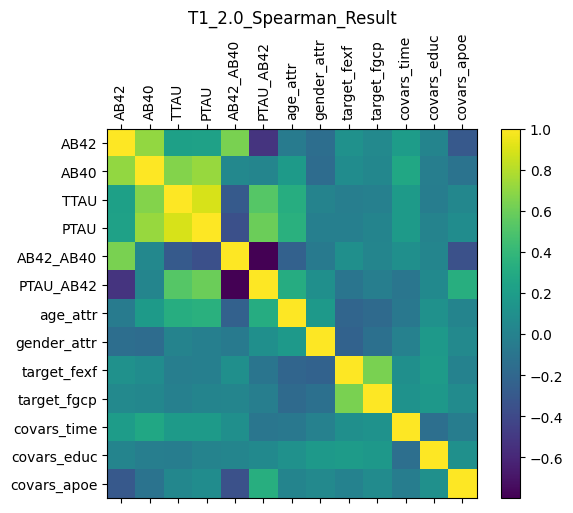
\includegraphics[width=0.24\textwidth]{chap6/figs/T1_2.0_Spearman_Result.png}
    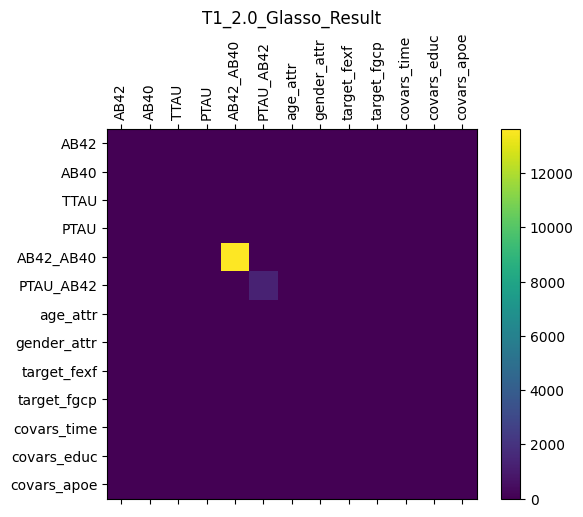
\includegraphics[width=0.24\textwidth]{chap6/figs/T1_2.0_Glasso_Result.png}
    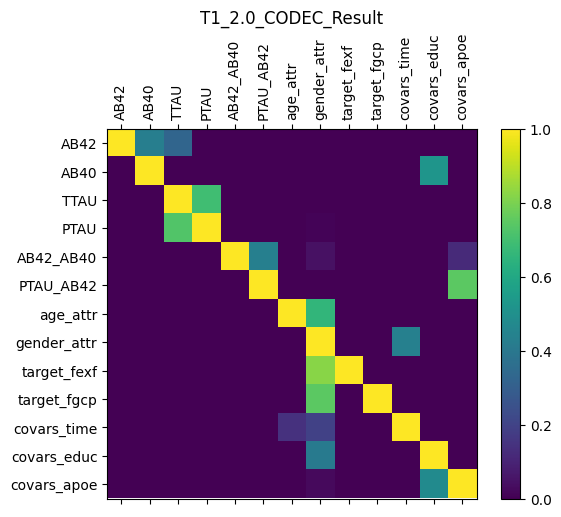
\includegraphics[width=0.24\textwidth]{chap6/figs/T1_2.0_CODEC_Result.png}
    
    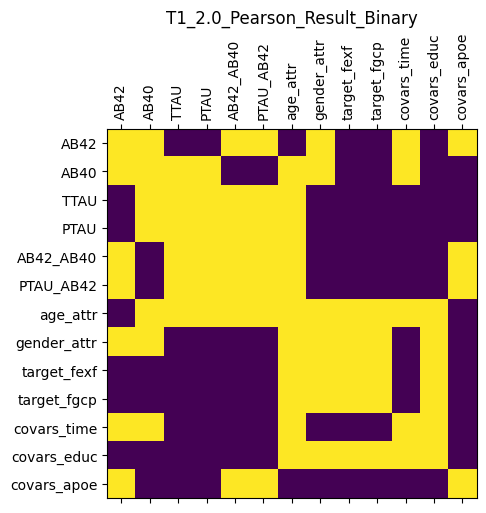
\includegraphics[width=0.24\textwidth]{chap6/figs/T1_2.0_Pearson_Result_Binary.png}
    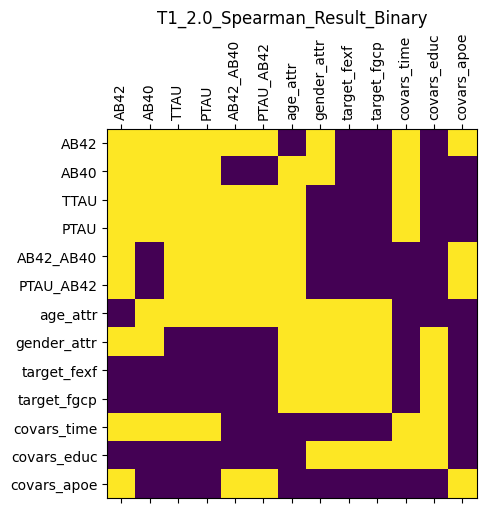
\includegraphics[width=0.24\textwidth]{chap6/figs/T1_2.0_Spearman_Result_Binary.png}
    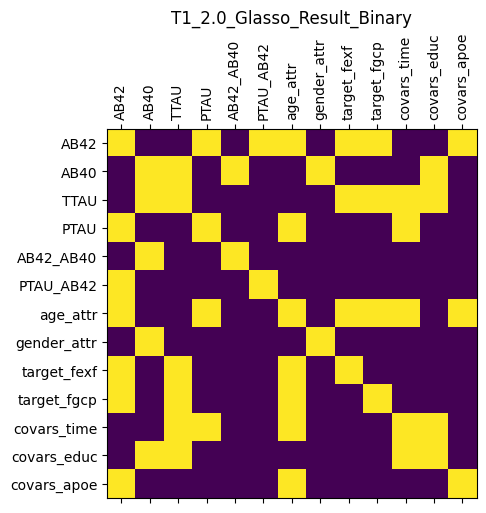
\includegraphics[width=0.24\textwidth]{chap6/figs/T1_2.0_Glasso_Result_Binary.png}
    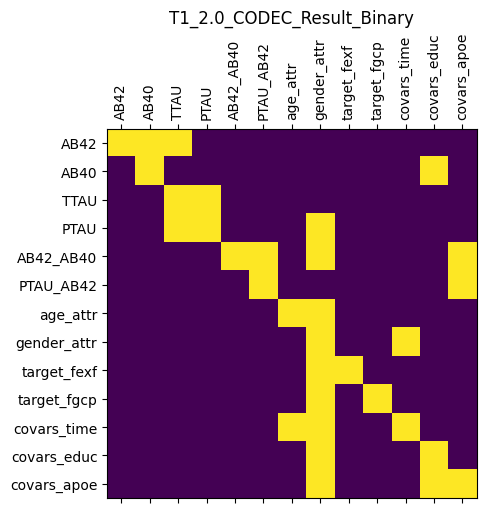
\includegraphics[width=0.24\textwidth]{chap6/figs/T1_2.0_CODEC_Result_Binary.png}
    \caption{Site 2: BIOCARD.}
    \label{fig:site2}
\end{figure}